\documentclass[main.tex]{subfiles}
\begin{document}

\section{Praktická část}
Hra je z velké části napsána v javascriptu, jenž dynamicky upravuje obsah html stránky. Ta je dále upravena pomocí css, aby připomínala starou herní konzoli. 

\subsection{Námět}
Hra se odehrává na palubě fiktivní rakety Shumaker-Levi 9, jenž je při startu neznámým způsobem poškozena, nicméně pokračuje dále v plánovaném letu. Komunikace hráče, jediného člena posádky, s řídicím střediskem je přerušena a hráč se tak ocitá v neznámým způsobem poškozené raketě a je nucen situaci vyřešit. 

Původní inspirací pro hru byla zkáza raketoplánu Columbia, která se odehrála 1. února 2003 při přistání. Příčinou havárie se ukázal být kousek hmoty, který se uvolnil při startu z externí palivové nádrže a udělal díru do křídla raketoplánu. Závada se projevila až při konci mise při přistání, kdy se do poškozeného křídla dostal horký vzduch, který poškodil statiku křídla, a raketoplán se rozpadl. \cite{web:wik:cz:columbia} 

Kvůli hře jednoho hráče byl raketoplán nahrazen raketou - rakeoplán je koncipován pro více osob. Děj hry je v blíže nespecifikovaných časových a místních podmínkách.

\subsection{Engine}
Samotnou hru zle rozdělit z hlediska funkčních celků na engine, který zajišťuje fungování hry - přijímání příkazů, vyhodnocování, reakce na nesprávné příkazy, chybové hlášky, atd., a samotný popis děje.
V enginu jsou implementovány pouze základní příkazy, které obecně fungují na větší množství objektů nebo hráče. Tím jsou myšleny přesuny mezi místnostmi, zvedání předmětů, nápovědy k lokalitám a předmětům, a také jejich popisy. Naproti tomu příkazy vztahující se k jednomu předmětu, například \textit{čti} jsou přesměrovány na konkrétní objekty (v případě přikazu \textit{čti} je to manuál), které je pak zpracují dle potřeby. To umožňuje snadnou a přehlednou rozšiřitelnost hry pomocí krátkých funkcí.

		\begin{figure}[h]
			\centering
			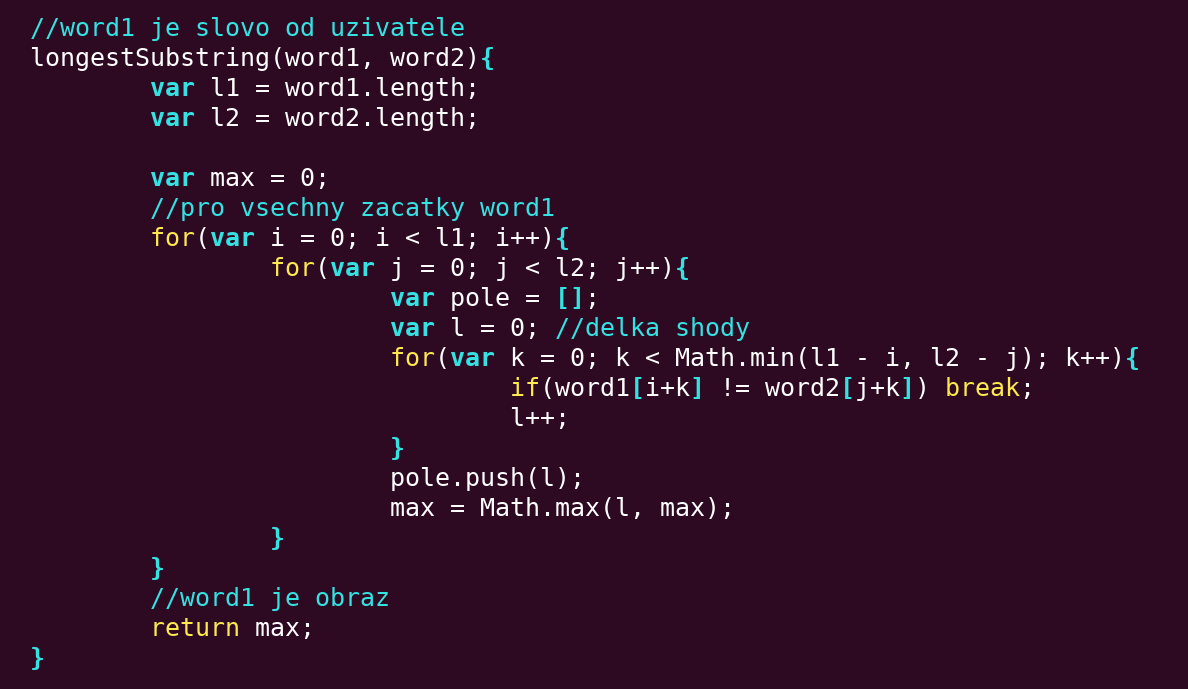
\includegraphics[width=.7\textwidth]{./praxe/longest_substring.png}
			\caption{Funkce na najití nejdelšího společného řetězce mezi vstupy }
		\end{figure}
Aby byl proces přidávání nových funkcí co nejjednoduší, jsou funkce zapsány v datové struktuře Map pod klíčem s jejich názvem. 

Příkaz přijatý od uživatele je nejprve upraven parserem, který najde odpovídající příkaz a poté je stromovou strukturou přesměrováván a zpracováván.

\subsection{Parsování vstupu}
Pro rozpoznávání uživatelem vložených příkazů slouží parser. Je-li vstup přijat od uživatele, parser jej nejprve zbaví diakritiky, poté je textový řetězec rozdělen na jednotlivá slova po mezerách. Tento proces je vykonán pří přijetí příkazu. Dále parser zajišťuje poznávání slov - nejprve ve funkci \textit{inputCommand} je příkaz rozdělený po mezerách testován s množinou názvů funkcí (jdi, pomoc, poloz, zvedni, popis, ...). V případě, že parser nerozpozná shodu mezi vstupem od uživatele a funkcemi, jsou dále takto testovány funkce u objektů. Je-li rozpoznána shoda s nějakou funkcí, je tato funkce zavolána. Uvnitř této funkce je opět testována shoda mezi předpokládanými parametry funkce (například příkaz \textit{jdi} očekává jako parametr název místnosti) a vstupem od uživatele. Tímto stromovým systémem je zpracováván celý vstup od uživatele, k čemuž napomáhá datová struktura Map.

		\begin{figure}[h]
			\centering
			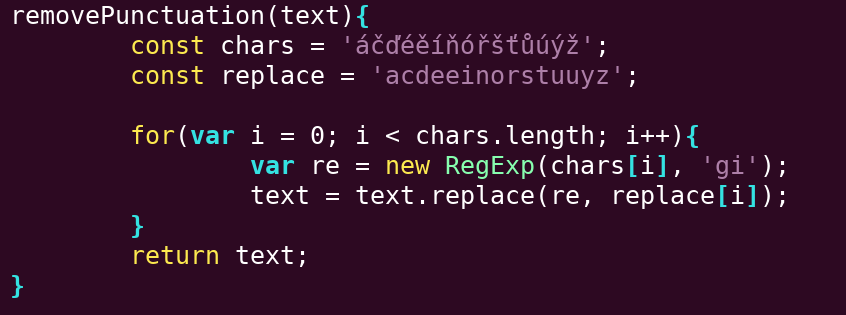
\includegraphics[width=.7\textwidth]{./praxe/remove_diacritics.png}
			\caption{Odstranění diakritiky ze vstupu}
		\end{figure}
\subsection{Příkazy}
Nyní budou stručně popsány příkazy, které jsou implementovány již v enginu, a jejich funkčnost.
\begin{itemize}
    \item popiš - tento příkaz, je-li zapsán bez parametrů, vypíše popis k aktuální místnosti. Pokud je s parametrem, popíše objekt, který mu byl zadán jako parametr, pokud je v dosahu. Synonymem je také \textit{rozhlédni se, prozkoumej}
    \item vezmi - příkaz vezmi přijímá parametr názvů objektů, které jsou v okolní místnosti. Pokud dostane jako parametr objekt, který se nenachází v okolní místnosti, vypíše chybovou hlášku. Je možné použít také slova \textit{zdvihni, zvedni, seber}.  
    \item polož - stejně jako příkaz vezmi, přijímá za parametry objekty, které si hráč nese s sebou. Zde je synonymem příkaz \textit{odlož}. 
    \item jdi - validními parametry jsou názvy místností. Zajišťuje přesun do sousedních místností. Dále je možno použít \textit{přesuň se}. 
\end{itemize}

		\begin{figure}[h]
			\centering
			
\includegraphics[width=.7\textwidth]{./praxe/uvod.png}
			%
\includegraphics[width=.7\textwidth]{./praxe/uvod.png}
			\caption{Po spuštění vítá hráče úvodní obrazovka}
		\end{figure}
\subsection{Děj}
Hra začíná startem rakety Shumaker-Levi 9, na jejíž palubě se hráč, jakožto vycvičený astronaut, ocitá. Při startu je však raketa neznámým způsobem poškozena a hráčovým úkolem se stává opravit raketu a vrátit se bezpečně na Zemi. Jediným pomocníkem se stává palubní manuál, v němž jsou popsány kroky, jenž musí hráč učinit, aby například prošel přechodovou komorou do volného vesmíru, kde zjistí rozsah poškození rakety. Manuál ve hře funguje jako jakýsi návod, k němuž by se měl hráč uchýlit v nouzi - neví-li jak postupovat. V manuálu jsou popsány netriviální a neintuitivní operace s předměty, které je potřeba učinit, aby hráč dosáhl pokroku. Příkladem může být samotné opravení závady, která, jak by měl hráč zjistit v průběhu hry, spočívá v poškozeném keramickém plášti rakety. Pro opravení pláště je potřeba vystoupit do vesmíru, kde je nutné přiložit na poškozené místo keramické destičky, které hráč najde v nákladovém prostoru, a následně je přišroubovat aku vrtačkou. Aku vrtačku najde hráč taktéž v nákladovém prostoru. Záludností ovšem je, že je zpočátku nenabitá, což by měl hráč zjistit až ve volném vesmíru, neboť v ostatních prostorech nelze, z důvodu bezpečnosti, aku vrtačku používat. K nabití slouží nabíječka, kterou hráč najde v kokpitu rakety. Tu je potřeba nejprve vzít do ruky, následně zapojit do nabíječky, a posléze nabít aku vrtačku. Nabíjení trvá několik minut. V této době by neměl hráč s nabíječkou nijak manipulovat (brát), neboť tím je proces nabíjení přerušen.  
		\begin{figure}[h]
			\centering
			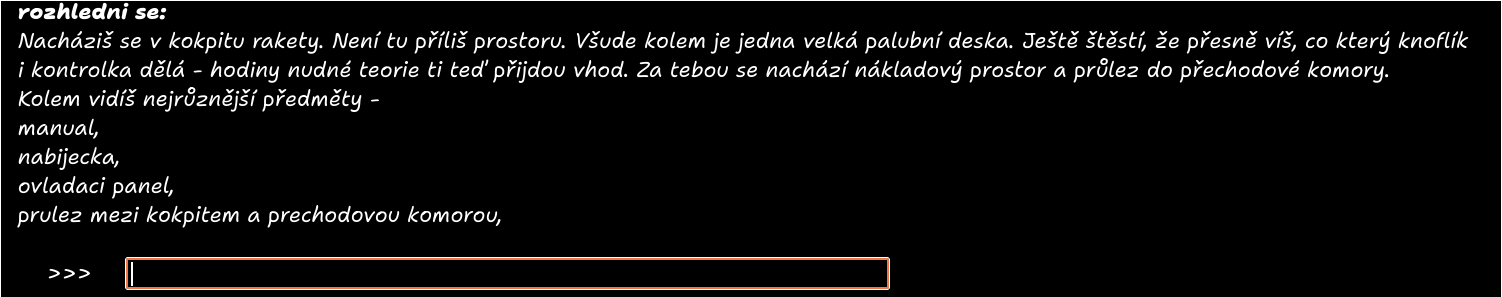
\includegraphics[width=1.0\textwidth]{./praxe/rozhledni.png}
			\caption{Po zadání příkazu rozhlédni se je vypsán popis okolí spolu s předměty v místnost.}
		\end{figure}


Hra se odehrává ve čtyřech lokalitách. Nejprve se hráč nachází v kokpitu, posléze objeví nákladový prostor, přechodovou komoru a volný vesmír. Lokality mají význam oddělení. Hráč tedy může používat pouze předměty, které má u sebe nebo se nacházejí ve stejné místnosti jako hráč. 

\end{document}

